\begin{examplebox}
\begin{minipage}{\linewidth}
\textbf{例1：圆在椭圆外，两条曲线外离。}
已知 $E:x^2/4+y^2=1$，$\Gamma:x^2+(y-4)^2=4$，求距离最值。
% E: x^2/4+y^2=1; Gamma: x^2+(y-4)^2=4. Equal metric scale.
\begin{center}
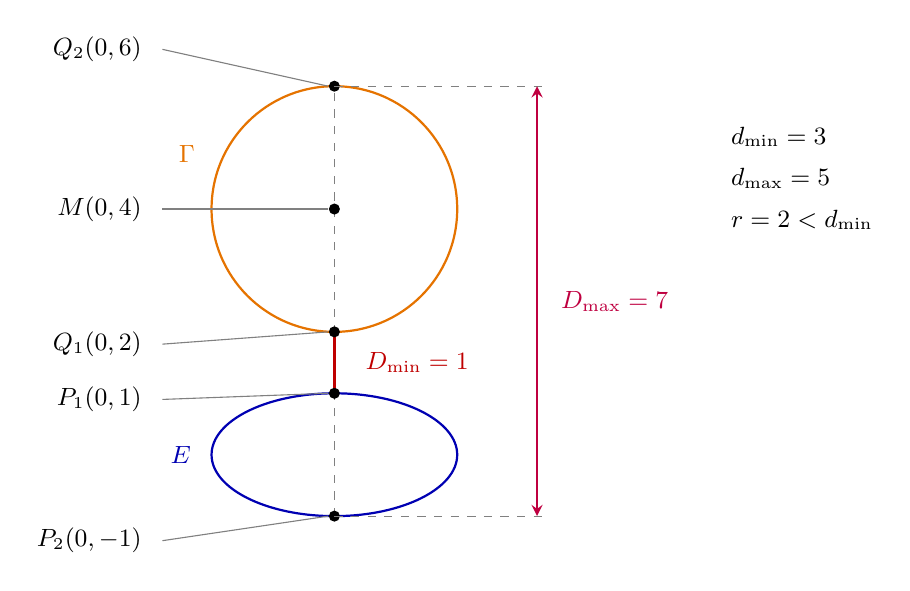
\begin{tikzpicture}[x=.78cm,y=.78cm,>=stealth,font=\small]
\draw[blue!70!black,thick] (0,0) ellipse (2 and 1);
\draw[orange!90!black,thick] (0,4) circle (2);
\node[blue!70!black] at (-2.5,0) {$E$};
\node[orange!90!black] at (-2.4,4.9) {$\Gamma$};
\draw[gray,dashed] (0,-1)--(0,6);
\draw[red!75!black,very thick] (0,1)--(0,2);
\foreach \yy in {1,2,-1,6,4} {\fill (0,\yy) circle(2pt);}
\draw[gray] (-.1,1)--(-2.8,.9) node[left=4pt,text=black] {$P_1(0,1)$};
\draw[gray] (-.1,2)--(-2.8,1.8) node[left=4pt,text=black] {$Q_1(0,2)$};
\draw[gray] (-.1,-1)--(-2.8,-1.4) node[left=4pt,text=black] {$P_2(0,-1)$};
\draw[gray] (-.1,6)--(-2.8,6.6) node[left=4pt,text=black] {$Q_2(0,6)$};
\draw[gray] (-.1,4)--(-2.8,4) node[left=4pt,text=black] {$M(0,4)$};
\node[red!75!black,anchor=west] at (.35,1.5) {$D_{\min}=1$};
\draw[gray,dashed] (0,-1)--(3.5,-1) (0,6)--(3.5,6);
\draw[<->,purple,thick] (3.3,-1)--(3.3,6)
 node[midway,right=5pt] {$D_{\max}=7$};
\node[anchor=west,align=left] at (6.3,4.5)
 {$d_{\min}=3$\\[4pt]$d_{\max}=5$\\[4pt]$r=2<d_{\min}$};
\end{tikzpicture}
\end{center}

\end{minipage}
\textbf{先求圆心距离范围。}令 $P=(2\cos\theta,\sin\theta)$，
$t=\sin\theta\in[-1,1]$，则
\[
 PM^2=4\cos^2\theta+(\sin\theta-4)^2=-3t^2-8t+20.
\]
对称轴 $t=-4/3$ 在区间左侧，且导数 $-6t-8<0$，故
\[
 d_{\min}=\sqrt{9}=3\quad(t=1),\qquad
 d_{\max}=\sqrt{25}=5\quad(t=-1).
\]
\textbf{再比较半径。}$r=2<3$，故
\[
 \boxed{D_{\min}=3-2=1,\qquad D_{\max}=5+2=7.}
\]
\textbf{图上回验：}$P_1(0,1),Q_1(0,2)$ 分别在两条曲线上，距离为1；
$P_2(0,-1),Q_2(0,6)$ 距离为7，与计算一致。
\end{examplebox}

\begin{examplebox}
\begin{minipage}{\linewidth}
\textbf{例2：两条曲线相交，距离最小值为零。}
已知 $E:x^2/4+y^2=1$，$\Gamma:(x-1)^2+y^2=4$，求距离最值。
% E: x^2/4+y^2=1; Gamma: (x-1)^2+y^2=4.
% Intersections x=(4-2sqrt(10))/3; y=+-sqrt(1-x^2/4).
\begin{center}
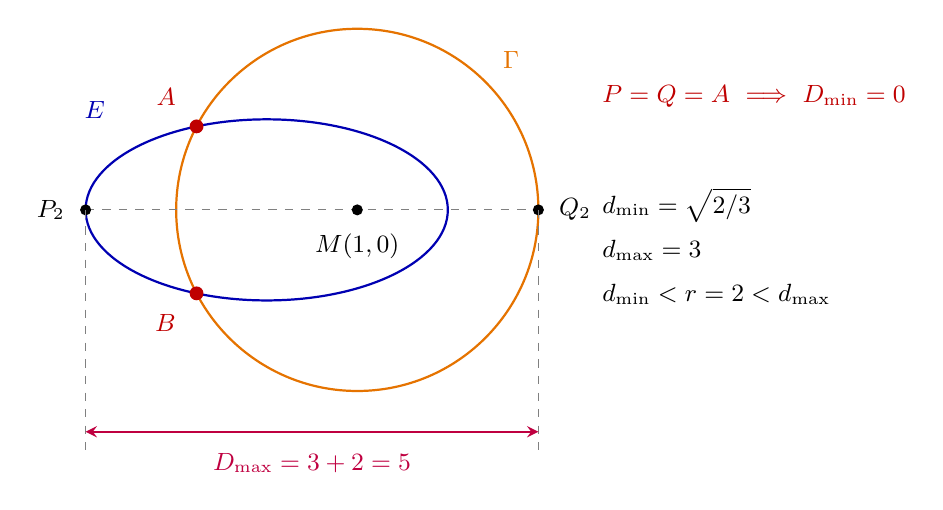
\begin{tikzpicture}[x=1.15cm,y=1.15cm,>=stealth,font=\small]
\pgfmathsetmacro{\ix}{(4-2*sqrt(10))/3}
\pgfmathsetmacro{\iy}{sqrt(1-\ix*\ix/4)}
\draw[blue!70!black,thick] (0,0) ellipse (2 and 1);
\draw[orange!90!black,thick] (1,0) circle (2);
\draw[gray,dashed] (-2,0)--(3,0);
\fill (1,0) circle(2pt) node[below=5pt] {$M(1,0)$};
\fill (-2,0) circle(2pt) node[left=4pt] {$P_2$};
\fill (3,0) circle(2pt) node[right=4pt] {$Q_2$};
\fill[red!75!black] (\ix,\iy) circle(2.5pt) node[above left=4pt] {$A$};
\fill[red!75!black] (\ix,-\iy) circle(2.5pt) node[below left=4pt] {$B$};
\node[red!75!black,anchor=west] at (3.6,1.25) {$P=Q=A\ \Longrightarrow\ D_{\min}=0$};
\node[blue!70!black] at (-1.9,1.1) {$E$};
\node[orange!90!black] at (2.7,1.65) {$\Gamma$};
\draw[gray,dashed] (-2,0)--(-2,-2.65) (3,0)--(3,-2.65);
\draw[<->,purple,thick] (-2,-2.45)--(3,-2.45)
 node[midway,below=4pt] {$D_{\max}=3+2=5$};
\node[anchor=west,align=left] at (3.6,-.4)
 {$d_{\min}=\sqrt{2/3}$\\[5pt]$d_{\max}=3$\\[5pt]$d_{\min}<r=2<d_{\max}$};
\end{tikzpicture}
\end{center}

\end{minipage}
\textbf{先求圆心距离范围。}令 $P=(2\cos\theta,\sin\theta)$，
$u=\cos\theta\in[-1,1]$，圆心为 $M(1,0)$，则
\[
 PM^2=(2u-1)^2+1-u^2=3u^2-4u+2
 =3\left(u-\frac23\right)^2+\frac23.
\]
最小值在 $u=2/3$ 处取得，最大值比较两端点得9，故
\[
 d_{\min}=\sqrt{\frac23},\qquad d_{\max}=3.
\]
\textbf{再比较半径。}$\sqrt{2/3}<r=2<3$，故
\[
 \boxed{D_{\min}=0,\qquad D_{\max}=3+2=5.}
\]
\textbf{图上回验：}联立方程得公共点
\[
 x_A=x_B=\frac{4-2\sqrt{10}}3,\qquad
 y_A=-y_B=\sqrt{1-\frac{x_A^2}{4}}.
\]
另一横坐标解 $(4+2\sqrt{10})/3>2$，不在椭圆上。
取 $P=Q=A$ 得距离0；取 $P_2(-2,0),Q_2(3,0)$ 得距离5。
\end{examplebox}

\begin{examplebox}
\begin{minipage}{\linewidth}
\textbf{例3：圆周包住椭圆，但两条边界的距离并不为零。}
已知 $E:x^2/4+y^2=1$，$\Gamma:x^2+(y+5)^2=64$，求距离最值。
% Example 3. E: x^2/4+y^2=1; Gamma: x^2+(y+5)^2=64.
\begin{center}
\begin{tikzpicture}[x=.48cm,y=.48cm,>=stealth,font=\small]
\draw[orange!90!black,thick] (0,-5) circle (8);
\draw[blue!70!black,thick] (0,0) ellipse (2 and 1);
\draw[gray,dashed] (0,-13)--(0,-10.2) (0,-6.5)--(0,3);
\draw[red!75!black,very thick] (0,1)--(0,3);
\fill (0,1) circle(2pt);
\draw[gray] (0,1)--(-2.5,-1)--(-4,-1.3);
\node[anchor=north] at (-4,-1.8) {$P(0,1)$};
\fill (0,3) circle(2pt) node[above=5pt] {$Q_1(0,3)$};
\fill (0,-13) circle(2pt) node[below=5pt] {$Q_2(0,-13)$};
\fill (0,-5) circle(2pt) node[left=6pt] {$M(0,-5)$};
\draw[gray,dashed] (0,3)--(9.3,3) (0,1)--(12.3,1) (0,-13)--(12.3,-13);
\draw[<->,red!75!black,thick] (9,1)--(9,3) node[midway,right=5pt] {$D_{\min}=2$};
\draw[<->,purple,thick] (12,1)--(12,-13) node[midway,right=5pt] {$D_{\max}=14$};
\node[blue!70!black] at (-3,-.8) {$E$};
\node[orange!90!black] at (-7.3,-.5) {$\Gamma$};
\node[align=left] at (0,-8.4) {$d_{\max}=MP=6<r=8$\\[5pt]到圆周有间隙，到圆盘为零};
\end{tikzpicture}
\end{center}

\end{minipage}
\textbf{先求圆心距离范围。}令 $t=\sin\theta\in[-1,1]$，
$P=(2\cos\theta,\sin\theta)$，圆心为 $M(0,-5)$，则
\[
 PM^2=4\cos^2\theta+(\sin\theta+5)^2=-3t^2+10t+29.
\]
导数 $-6t+10>0$，故最小、最大值分别在 $t=-1,1$ 处取得：
\[
 d_{\min}=\sqrt{16}=4,\qquad d_{\max}=\sqrt{36}=6.
\]
\textbf{再比较半径。}$r=8>d_{\max}=6$，故
\[
 \boxed{D_{\min}=8-6=2,\qquad D_{\max}=6+8=14.}
\]
\textbf{图上回验：}椭圆点 $P(0,1)$ 与圆周点 $Q_1(0,3)$ 距离为2，
与圆周点 $Q_2(0,-13)$ 距离为14。三点均满足各自方程。
最近点和最远点这两组配对，使用的是\textbf{同一个椭圆点} $P$。
\end{examplebox}
